\begin{frame}
\frametitle{3D exemple: a cantilever beam}

\begin{itemize}
\item The vertical deflection $y$ of a cantilever beam's free end of fixed length $L$ reads as
\[ y=\frac{FL^3}{3EI}, \]
where:
\begin{itemize}
\item $E$ is the Young modulus; 
\item $F$ is the load;
\item $I$ is the moment of inertia.
\end{itemize}

\item \textit{Input} variables $x=(F,E,I)$ are assumed random;

\item Variable of interest (\textit{output}) is the deflection $y$ estimated thanks to the model $\mathcal{M}$
\[ \mathcal{M}: x \mapsto y\]

\item Building a metamodel $\tilde{\mathcal{M}}$ through Kriging and optimization loop for parameters: one \hmat at each iteration to treat the covariance matrix associated with a specified covariance model.
\end{itemize}

\end{frame}

\begin{frame}[fragile]

 The chosen covariance model $K_{\lambda}(s,t)$ is the following tensor product:
\[ e^{-(s_1-t_1)/\lambda_1} e^{-(s_2-t_2)/\lambda_2} e^{-(s_3-t_3)/\lambda_3}. \]
\begin{itemize}
\item Let $\lambda_1 = 3.96528$, $\lambda_2 = 5.8237$ and $\lambda_3 = 9.0679$ be the starting coefficients for the optimization.

\item Degrees of freedom to be clustered within the \hmat framework:
\begin{lstlisting}
"Young modulus";"Load";"Inertia" 
3.6258375026+07;4.797336026+04;3.5171332517+02
3.1382130227+07;3.350317520+04;3.5324327901+02
... ... ... ... ... ... ... ... ... ... ... ..
\end{lstlisting}
\end{itemize}
\end{frame}

\begin{frame}
\frametitle{Results}

\only<1|handout:3>{
\begin{figure}[H]
\begin{center}
  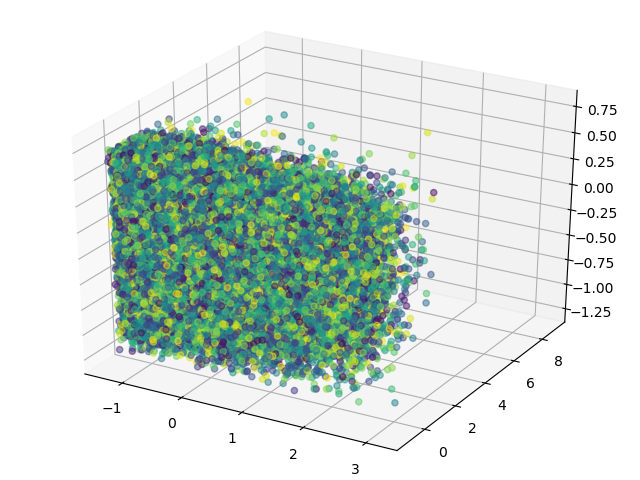
\includegraphics[scale=0.4]{./img/scatter}
  \caption{Input data: $5 \times 10^{4}$ entries.}
\end{center}
\end{figure}
\begin{itemize}
\item covariance matrix of size $5.10^{4} \times 5.10^{4}$, symmetric and double precision: full size in memory is $10 \mathrm{Go}$.
\end{itemize}
}
\only<2|handout:3>{
\begin{figure}[H]
\begin{center}
  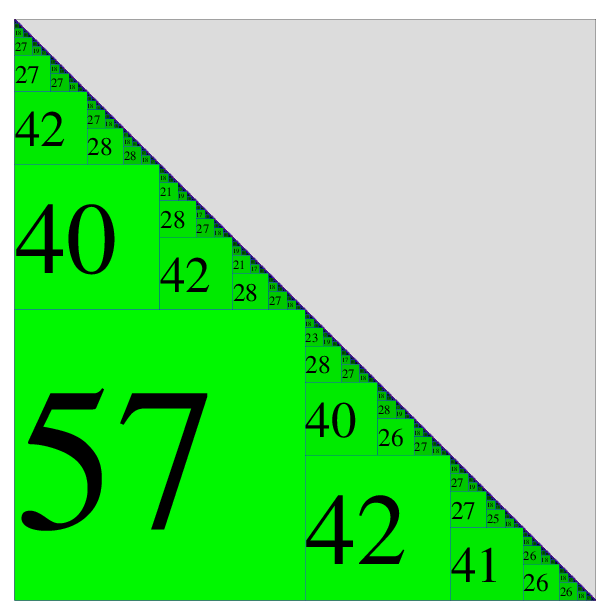
\includegraphics[scale=0.23]{./img/hmatrix_assembled}
  \caption{Lower part of the covariance matrix: rank map.}
\end{center}
\end{figure}

\begin{itemize}
\item memory: $167\mathrm{Mo}$ (compression ratio: 1.67\%);
\item assembly time: $11.83\mathrm{s}$
\end{itemize}

}
\only<3|handout:3>{
\begin{figure}[H]
\begin{center}
  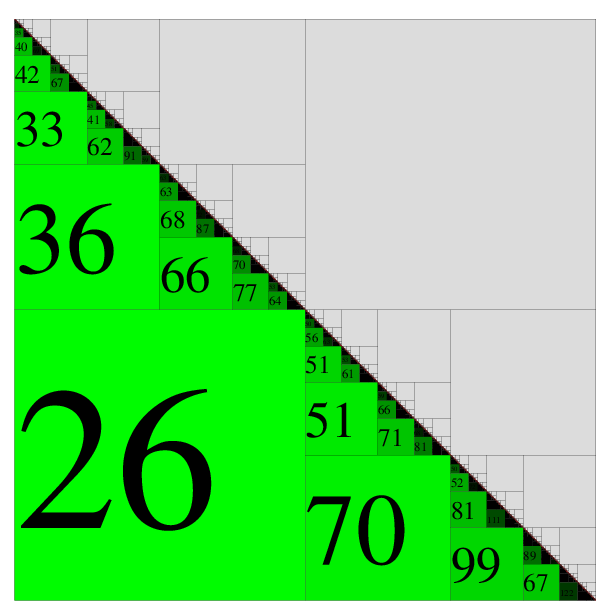
\includegraphics[scale=0.23]{./img/hmatrix_factorized}
  \caption{Cholesky factor: rank map.}
\end{center}
\end{figure}
\begin{itemize}
\item memory: $263\mathrm{Mo}$ (compression ratio: 2.63\%);
\item Cholesky time: $17.84\mathrm{s}$
\end{itemize}
}

\end{frame}

\begin{frame}
\frametitle{Gaussian process}
\begin{figure}[H]
\begin{center}
  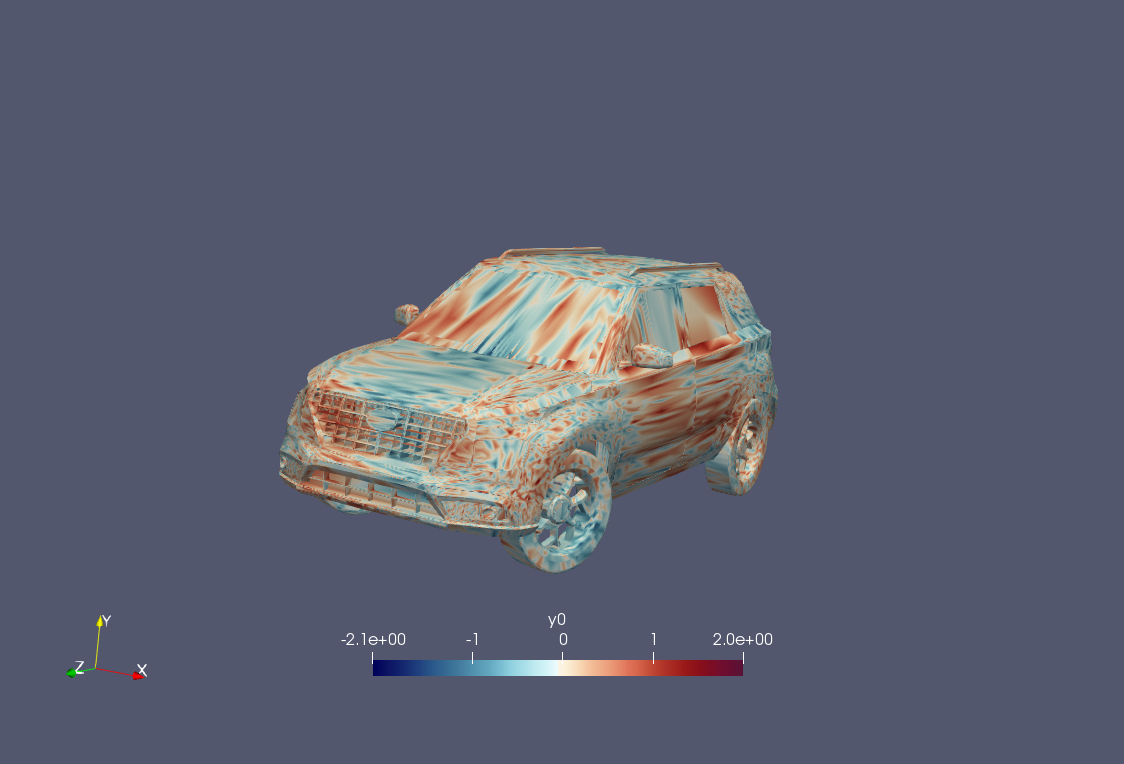
\includegraphics[scale=0.15]{./img/voiture}
  \caption{A Gaussian process on a Hyundai FEM mesh}
\end{center}
\end{figure}
\begin{itemize}
\item $144966$ vertices;
\item squared exponential covariance kernel.
\item Build, Cholesky factorization and trajectory generation in 118s.
\end{itemize}
\end{frame}
